
% --- SLIDE 5: PRUNING ---
\begin{frame}{Pruning: Stop Wasting Compute on Hopeless Trials}

    \centering
    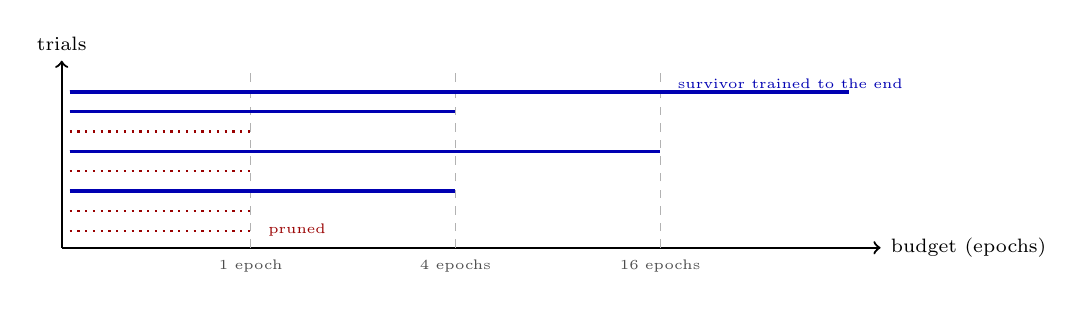
\begin{tikzpicture}[
        yscale=0.72,
        font=\scriptsize,
        rung/.style={draw, dashed, gray!60},
        alive/.style={very thick, blue!70!black},
        dead/.style={thick, red!60!black, dotted}
    ]
        % axes
        \draw[->, thick] (0,0) -- (10.4,0) node[right, font=\scriptsize] {budget (epochs)};
        \draw[->, thick] (0,0) -- (0,3.3) node[above, font=\scriptsize] {trials};

        % rung markers
        \foreach \x/\lab in {2.4/{1 epoch}, 5.0/{4 epochs}, 7.6/{16 epochs}} {
            \draw[rung] (\x,0) -- (\x,3.1);
            \node[gray!60!black, font=\tiny, anchor=north] at (\x,-0.05) {\lab};
        }

        % 8 trials start, 4 pass rung 1, 2 pass rung 2, 1 passes rung 3
        \foreach \y in {0.3,0.65,1.0,1.35,1.7,2.05,2.4,2.75}
            \draw[dead] (0.1,\y) -- (2.4,\y);
        \foreach \y in {1.0,1.7,2.4,2.75}
            \draw[alive] (0.1,\y) -- (5.0,\y);
        \foreach \y in {1.7,2.75}
            \draw[alive] (0.1,\y) -- (7.6,\y);
        \draw[alive] (0.1,2.75) -- (10.0,2.75);

        \node[red!60!black, font=\tiny, anchor=west] at (2.5,0.32) {pruned};
        \node[blue!70!black, font=\tiny, anchor=west] at (7.7,2.9) {survivor trained to the end};
    \end{tikzpicture}

    \vspace{0.05em}
    \begin{columns}[T]
        \begin{column}{0.5\textwidth}
            \scriptsize
            \textbf{Successive halving / ASHA}
            \begin{itemize}
                \item Give every trial a small budget. At each ``rung'', promote only the top
                      $1/\eta$ and kill the rest.
                \item Optuna's \texttt{SuccessiveHalvingPruner} implements the \emph{asynchronous} version
                      (ASHA): a trial is promoted as soon as it qualifies, so workers never idle.
                \item Default reduction factor $\eta = 4$.
            \end{itemize}
        \end{column}
        \begin{column}{0.46\textwidth}
            \scriptsize
            \textbf{Which pruner}
            \begin{itemize}
                \item \texttt{MedianPruner} --- Optuna's default. Prune if you are below the median of
                      finished trials at this step. Gentle, safe.
                \item \texttt{SuccessiveHalvingPruner} --- aggressive, best under a fixed wall-clock budget.
                \item \texttt{HyperbandPruner} --- runs successive halving at several starting budgets to
                      hedge the ``too aggressive'' risk.
            \end{itemize}
        \end{column}
    \end{columns}

    \vspace{0.04em}
    {\scriptsize Sources: Optuna documentation, \href{https://optuna.readthedocs.io/en/stable/reference/generated/optuna.pruners.SuccessiveHalvingPruner.html}{\texttt{SuccessiveHalvingPruner}};
    Li et al., ``A System for Massively Parallel Hyperparameter Tuning,'' MLSys 2020, \href{https://arxiv.org/abs/1810.05934v5}{arXiv:1810.05934v5};
    Li et al., ``Hyperband,'' \textit{JMLR} 18, 2018, \href{https://arxiv.org/abs/1603.06560v4}{arXiv:1603.06560v4}.}

\end{frame}
